\documentclass[border=3pt]{standalone}
% Preâmbulo compartilhado pelos diagramas TikZ da aula 8 de IHR (Métodos de Pesquisa)
\usepackage[T1]{fontenc}
\usepackage[utf8]{inputenc}
\usepackage{lmodern}
\usepackage{amsmath}
\usepackage{xcolor}
\usepackage{tikz}
\usetikzlibrary{arrows.meta,angles,quotes,decorations.pathmorphing,decorations.pathreplacing,calc,
                positioning,shapes.geometric,shapes.misc,backgrounds,fit,
                math}

% Paleta (mesma dos SVGs originais)
% Paleta da disciplina de IHR: acento azul (#1A6FB5), cor de destaque do tema.
% (o nome "dblue" é mantido para não alterar todos os diagramas)
\definecolor{dblue}{HTML}{1A6FB5}
\definecolor{dorange}{HTML}{B3541E}
\definecolor{dgreen}{HTML}{4A7C59}
\definecolor{dred}{HTML}{9C4B4B}
\definecolor{dcream}{HTML}{F4F1EA}
\definecolor{dshade}{HTML}{DDD7C9}

% Função gaussiana (não normalizada por padrão de escala visual)
\pgfmathdeclarefunction{gauss}{3}{%
  \pgfmathparse{1/(#3*sqrt(2*pi))*exp(-((#1-#2)^2)/(2*#3^2))}%
}

% Estilos comuns (prefixo d... para não colidir com chaves internas do pgf)
\tikzset{
  >={Stealth[length=2mm]},
  dguide/.style={gray!55, dashed, line width=0.4pt},
  daxis/.style={gray!60, line width=0.7pt, ->},
  dbody/.style={fill=black!3, draw=black!80, line width=1pt},
  dacc/.style={draw=dblue, line width=1pt},
  dlbl/.style={black!55, font=\small},
  dsub/.style={black!45, font=\footnotesize},
  dstate/.style={circle, draw=black!80, fill=dcream, line width=1pt,
                 minimum size=17mm, font=\large, inner sep=1pt},
  dobs/.style={circle, draw=black!80, fill=dshade, line width=1pt,
               minimum size=14mm, font=\large, inner sep=1pt},
  dbox/.style={rounded corners=2pt, draw=black!80, fill=dcream, line width=1pt,
               align=center, inner sep=6pt},
  dop/.style={circle, draw=black!80, fill=white, line width=1pt,
              minimum size=6mm, inner sep=0pt, font=\small},
  dtrans/.style={->, dblue, line width=1pt},
  dmeas/.style={->, dorange, line width=1pt},
  dcurve/.style={line width=1pt, dblue},
  dcurveb/.style={line width=1.4pt, dorange},
}

\begin{document}
\hyphenpenalty=10000 \exhyphenpenalty=10000 \tolerance=9999 \emergencystretch=3em
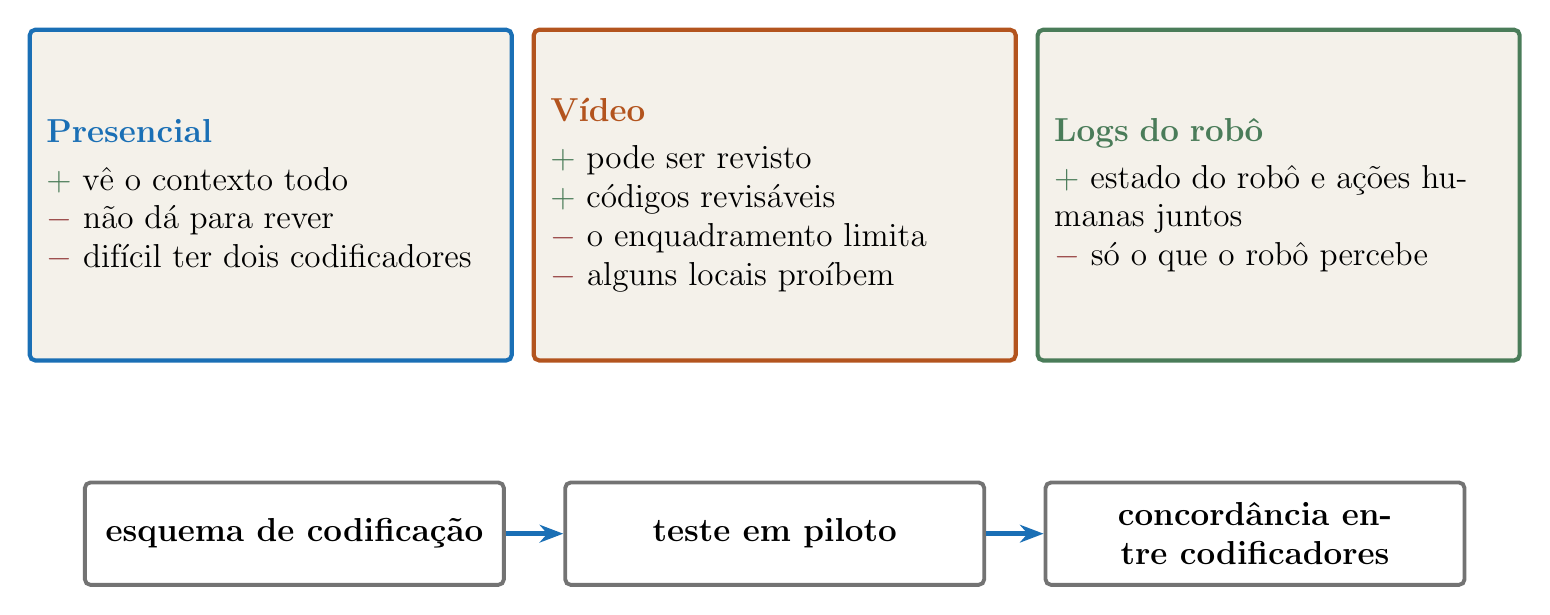
\begin{tikzpicture}[x=1cm,y=1cm]
  \tikzset{c/.style={dbox, text width=5.7cm, minimum height=4.2cm, font=\large, line width=1.5pt, align=left}}
  \node[c, draw=dblue] at (3.1,5.7) {\textbf{\textcolor{dblue}{Presencial}}\\[3pt] \textcolor{dgreen}{$+$} vê o contexto todo\\ \textcolor{dred}{$-$} não dá para rever\\ \textcolor{dred}{$-$} difícil ter dois codificadores};
  \node[c, draw=dorange] at (9.5,5.7) {\textbf{\textcolor{dorange}{Vídeo}}\\[3pt] \textcolor{dgreen}{$+$} pode ser revisto\\ \textcolor{dgreen}{$+$} códigos revisáveis\\ \textcolor{dred}{$-$} o enquadramento limita\\ \textcolor{dred}{$-$} alguns locais proíbem};
  \node[c, draw=dgreen] at (15.9,5.7) {\textbf{\textcolor{dgreen}{Logs do robô}}\\[3pt] \textcolor{dgreen}{$+$} estado do robô e ações humanas juntos\\ \textcolor{dred}{$-$} só o que o robô percebe};
  \tikzset{e/.style={dbox, draw=black!55, fill=white, line width=1.4pt, text width=4.9cm, minimum height=1.3cm, font=\large\bfseries, align=center}}
  \node[e] (x) at (3.4,1.4) {esquema de codificação};
  \node[e] (y) at (9.5,1.4) {teste em piloto};
  \node[e] (z) at (15.6,1.4) {concordância entre codificadores};
  \draw[dtrans, line width=1.8pt, -{Stealth[length=3mm]}] (x.east) -- (y.west);
  \draw[dtrans, line width=1.8pt, -{Stealth[length=3mm]}] (y.east) -- (z.west);
\end{tikzpicture}
\end{document}
